% Template Created by Albert Alises Sorribas (albert.alises@gmail.com) for the thesis of the MSc. in Computational Biomedical Engineering, Universitat Pompeu Fabra. Based on the thesis template of the Imperial College London,  downloadable at http://www.imperial.ac.uk/brand-style-guide/templates/downloadable-templates/

\documentclass[a4paper,12pt,twoside]{report}
\usepackage[left=3cm,right=3cm,top=3cm,bottom=3cm]{geometry} %Margins
\usepackage{pdfpages}
\usepackage{hyperref}
\usepackage{listings}
\usepackage{xcolor}
\usepackage{setspace}
\usepackage{tocloft}
\usepackage{amsmath}
\usepackage{chngcntr }
\usepackage[toc,page]{appendix}
\usepackage[T1]{fontenc}
\usepackage[nottoc]{tocbibind}
\usepackage[compact]{titlesec}
\titlespacing{\section}{0pt}{1ex}{0ex}
\titlespacing{\subsection}{0pt}{1ex}{0ex}
\titlespacing{\subsubsection}{0pt}{1ex}{0ex}

\counterwithout{figure}{chapter}
\counterwithout{table}{chapter}

\usepackage{graphicx}
\usepackage{verbatim}
\usepackage{latexsym}
\def\bbbr{{\rm I\!R}} %reelle Zahlen
\def\bbbm{{\rm I\!M}}
\def\bbbn{{\rm I\!N}} %natuerliche Zahlen
\def\bbbf{{\rm I\!F}}
\def\bbbh{{\rm I\!H}}
\def\bbbk{{\rm I\!K}}
\def\bbbp{{\rm I\!P}}
\def\bbbe{{\rm I\!E}}
\def\bbbone{{\mathchoice {\rm 1\mskip-4mu l} {\rm 1\mskip-4mu l}
{\rm 1\mskip-4.5mu l} {\rm 1\mskip-5mu l}}}
\def\bbbc{{\mathchoice {\setbox0=\hbox{$\displaystyle\rm C$}\hbox{\hbox
to0pt{\kern0.4\wd0\vrule height0.9\ht0\hss}\box0}}
{\setbox0=\hbox{$\textstyle\rm C$}\hbox{\hbox
to0pt{\kern0.4\wd0\vrule height0.9\ht0\hss}\box0}}
{\setbox0=\hbox{$\scriptstyle\rm C$}\hbox{\hbox
to0pt{\kern0.4\wd0\vrule height0.9\ht0\hss}\box0}}
{\setbox0=\hbox{$\scriptscriptstyle\rm C$}\hbox{\hbox
to0pt{\kern0.4\wd0\vrule height0.9\ht0\hss}\box0}}}}
\def\bbbq{{\mathchoice {\setbox0=\hbox{$\displaystyle\rm
Q$}\hbox{\raise
0.15\ht0\hbox to0pt{\kern0.4\wd0\vrule height0.8\ht0\hss}\box0}}
{\setbox0=\hbox{$\textstyle\rm Q$}\hbox{\raise
0.15\ht0\hbox to0pt{\kern0.4\wd0\vrule height0.8\ht0\hss}\box0}}
{\setbox0=\hbox{$\scriptstyle\rm Q$}\hbox{\raise
0.15\ht0\hbox to0pt{\kern0.4\wd0\vrule height0.7\ht0\hss}\box0}}
{\setbox0=\hbox{$\scriptscriptstyle\rm Q$}\hbox{\raise
0.15\ht0\hbox to0pt{\kern0.4\wd0\vrule height0.7\ht0\hss}\box0}}}}
\def\bbbt{{\mathchoice {\setbox0=\hbox{$\displaystyle\rm
T$}\hbox{\hbox to0pt{\kern0.3\wd0\vrule height0.9\ht0\hss}\box0}}
{\setbox0=\hbox{$\textstyle\rm T$}\hbox{\hbox
to0pt{\kern0.3\wd0\vrule height0.9\ht0\hss}\box0}}
{\setbox0=\hbox{$\scriptstyle\rm T$}\hbox{\hbox
to0pt{\kern0.3\wd0\vrule height0.9\ht0\hss}\box0}}
{\setbox0=\hbox{$\scriptscriptstyle\rm T$}\hbox{\hbox
to0pt{\kern0.3\wd0\vrule height0.9\ht0\hss}\box0}}}}
\def\bbbs{{\mathchoice
{\setbox0=\hbox{$\displaystyle     \rm S$}\hbox{\raise0.5\ht0\hbox
to0pt{\kern0.35\wd0\vrule height0.45\ht0\hss}\hbox
to0pt{\kern0.55\wd0\vrule height0.5\ht0\hss}\box0}}
{\setbox0=\hbox{$\textstyle        \rm S$}\hbox{\raise0.5\ht0\hbox
to0pt{\kern0.35\wd0\vrule height0.45\ht0\hss}\hbox
to0pt{\kern0.55\wd0\vrule height0.5\ht0\hss}\box0}}
{\setbox0=\hbox{$\scriptstyle      \rm S$}\hbox{\raise0.5\ht0\hbox
to0pt{\kern0.35\wd0\vrule height0.45\ht0\hss}\raise0.05\ht0\hbox
to0pt{\kern0.5\wd0\vrule height0.45\ht0\hss}\box0}}
{\setbox0=\hbox{$\scriptscriptstyle\rm S$}\hbox{\raise0.5\ht0\hbox
to0pt{\kern0.4\wd0\vrule height0.45\ht0\hss}\raise0.05\ht0\hbox
to0pt{\kern0.55\wd0\vrule height0.45\ht0\hss}\box0}}}}
\def\bbbz{{\mathchoice {\hbox{$\mathsf\textstyle Z\kern-0.4em Z$}}
{\hbox{$\mathsf\textstyle Z\kern-0.4em Z$}}
{\hbox{$\mathsf\scriptstyle Z\kern-0.3em Z$}}
{\hbox{$\mathsf\scriptscriptstyle Z\kern-0.2em Z$}}}}
\usepackage{setspace}
\usepackage{blindtext}
\usepackage{float}

\setlength{\parskip}{\medskipamount}  % a little space before a \par
\setlength{\parindent}{0pt}	      % don't indent first lines of paragraphs
%UHEAD.STY  If this is included after \documentstyle{report}, it adds
% an underlined heading style to the LaTeX report style.
% \pagestyle{uheadings} will put underlined headings at the top
% of each page. The right page headings are the Chapter titles and
% the left page titles are supplied by \def\lefthead{text}.

% Ted Shapin, Dec. 17, 1986

\makeatletter
\def\chapapp2{Chapter}

\def\appendix{\par
 \setcounter{chapter}{0}
 \setcounter{section}{0}
 \def\chapapp2{Appendix}
 \def\@chapapp{Appendix}
 \def\thechapter{\Alph{chapter}}}

\def\ps@uheadings{\let\@mkboth\markboth
% modifications
\def\@oddhead{\protect\underline{\protect\makebox[\textwidth][l]
		{\sl\rightmark\hfill\rm\thepage}}}
\def\@oddfoot{}
\def\@evenfoot{}
\def\@evenhead{\protect\underline{\protect\makebox[\textwidth][l]
		{\rm\thepage\hfill\sl\leftmark}}}
% end of modifications
\def\chaptermark##1{\markboth {\ifnum \c@secnumdepth >\m@ne
 \chapapp2\ \thechapter. \ \fi ##1}{}}%
\def\sectionmark##1{\markright {\ifnum \c@secnumdepth >\z@
   \thesection. \ \fi ##1}}}
\makeatother
%%From: marcel@cs.caltech.edu (Marcel van der Goot)
%%Newsgroups: comp.text.tex
%%Subject: illegal modification of boxit.sty
%%Date: 28 Feb 92 01:10:02 GMT
%%Organization: California Institute of Technology (CS dept)
%%Nntp-Posting-Host: andromeda.cs.caltech.edu
%%
%%
%%Quite some time ago I posted a file boxit.sty; maybe it made it
%%to some archives, although I don't recall submitting it. It defines
%%	\begin{boxit}
%%	...
%%	\end{boxit}
%%to draw a box around `...', where the `...' can contain other
%%environments (e.g., a verbatim environment). Unfortunately, it had
%%a problem: it did not work if you used it in paragraph mode, i.e., it
%%only worked if there was an empty line in front of \begin{boxit}.
%%Luckily, that is easily corrected.
%%
%%HOWEVER, apparently someone noticed the problem, tried to correct it,
%%and then distributed this modified version. That would be fine with me,
%%except that:
%%1. There was no note in the file about this modification, it only has my
%%   name in it.
%%2. The modification is wrong: now it only works if there is *no* empty
%%   line in front of \begin{boxit}. In my opinion this bug is worse than
%%   the original one.
%%
%%In particular, the author of this modification tried to force an empty
%%line by inserting a `\\' in the definition of \Beginboxit. If you have
%%a version of boxit.sty with a `\\', please delete it. If you have my
%%old version of boxit.sty, please also delete it. Below is an improved
%%version.
%%
%%Thanks to Joe Armstrong for drawing my attention to the bug and to the
%%illegal version.
%%
%%                                          Marcel van der Goot
%% .---------------------------------------------------------------
%% | Blauw de viooltjes,                    marcel@cs.caltech.edu
%% |    Rood zijn de rozen;
%% | Een rijm kan gezet
%% |    Met plaksel en dozen.
%% |


% boxit.sty
% version: 27 Feb 1992
%
% Defines a boxit environment, which draws lines around its contents.
% Usage:
%   \begin{boxit}
%	... (text you want to be boxed, can contain other environments)
%   \end{boxit}
%
% The width of the box is the width of the contents.
% The boxit* environment behaves the same, except that the box will be
% at least as wide as a normal paragraph.
%
% The reason for writing it this way (rather than with the \boxit#1 macro
% from the TeXbook), is that now you can box verbatim text, as in
%   \begin{boxit}
%   \begin{verbatim}
%   this better come out in boxed verbatim mode ...
%   \end{verbatim}
%   \end{boxit}
%
%						Marcel van der Goot
%						marcel@cs.caltech.edu
%

\def\Beginboxit
   {\par
    \vbox\bgroup
	   \hrule
	   \hbox\bgroup
		  \vrule \kern1.2pt %
		  \vbox\bgroup\kern1.2pt
   }

\def\Endboxit{%
			      \kern1.2pt
		       \egroup
		  \kern1.2pt\vrule
		\egroup
	   \hrule
	 \egroup
   }	

\newenvironment{boxit}{\Beginboxit}{\Endboxit}
\newenvironment{boxit*}{\Beginboxit\hbox to\hsize{}}{\Endboxit}
\pagestyle{empty}

\setlength{\parskip}{2ex plus 0.5ex minus 0.2ex}
\setlength{\parindent}{0pt}

\makeatletter  %to avoid error messages generated by "\@". Makes Latex treat "@" like a letter

\linespread{1.5}
\def\submitdate#1{\gdef\@submitdate{#1}}
\def\supervisor#1{\gdef\@supervisor{#1}}
\def\cosupervisor#1{\gdef\@cosupervisor{#1}}

\def\maketitle{
  % Title
  \begin{titlepage}{
    \vspace*{2\baselineskip} %Empty Lines
    {\fontsize{17.28}{16.8}\selectfont Master thesis Sound and Music Computing}\\
     {\fontsize{14}{16.8}\selectfont Universitat Pompeu Fabra}\\
    \rm
    \vspace*{3\baselineskip} %Empty Lines
     \bf \fontsize{24.88}{17.5}\selectfont  \@title \par
  }
  \vskip 0.3in
  \par
  {\fontsize{14}{27}\selectfont  \@author}

  \vskip 0.20in
  \fontsize{14}{16.8}\selectfont \textbf{Supervisor:}   \@supervisor \\
  \fontsize{14}{16.8}\selectfont \textbf{Co-Supervisor:}  \@cosupervisor \\
   \vspace*{3\baselineskip} %Empty Lines
    \fontsize{14}{27}\selectfont  \@submitdate \\
    \vspace{ 0.7in}
    
\includegraphics[width=8cm]{Figures/LogoPompeuFabra}\\[.5cm]
  \vfil
  \end{titlepage}
}

\def\titlepage{
  \newpage
  \centering
  \linespread{1.5}
  \normalsize
  \vbox to \vsize\bgroup\vbox to 9in\bgroup
}
\def\endtitlepage{
  \par
  \kern 0pt
  \egroup
  \vss
  \egroup
  \cleardoublepage
}

\def\abstract{
  \begin{center}{
    \large\bf Abstract}
  \end{center}
  \small
  %\def\baselinestretch{1.5}
  \linespread{1.5}
  \normalsize
}
\def\endabstract{
  \par
   \cleardoublepage
}

\newenvironment{acknowledgement}{
  \clearpage
  \begin{center}{
    \large \bf Acknowledgement}
  \end{center}
  \small
  \linespread{1.5}
  \normalsize
}{\clearpage}
\def\endacknowledgement{
  \par
    \cleardoublepage
}

\newenvironment{dedication}{
  \clearpage
  \begin{center}{
    \large \bf Dedication}
  \end{center}
  \small
  \linespread{1.5}
  \normalsize
}{\clearpage}
\def\enddedication{
  \par
  \cleardoublepage
}

\def\preface{
    \pagenumbering{gobble}
    \pagestyle{plain}
    \doublespacing
     \setcounter{tocdepth}{2}
    \tableofcontents
}

\def\body{

    \clearpage
    \pagestyle{uheadings}
    \pagenumbering{arabic}
    \singlespacing
    \setlength{\cftbeforesecskip}{10pt}

    \pagestyle{plain}
    \clearpage
    \pagestyle{uheadings}

}

\makeatother  %to avoid error messages generated by "\@". Makes Latex treat "@" like a letter


\newcommand{\titlelinespacing}{\renewcommand{\baselinestretch}{2.0} \normalsize}
\newcommand{\normallinespacing}{\renewcommand{\baselinestretch}{1.5} \normalsize}
\newcommand{\mediumlinespacing}{\renewcommand{\baselinestretch}{1.2} \normalsize}
\newcommand{\narrowlinespacing}{\renewcommand{\baselinestretch}{1.0} \normalsize}

\newtheorem{definition}{Definition}[chapter]
\newtheorem{theorem}{Theorem}[chapter]
\cftsetindents{section}{0in}{0.5in}
\cftsetindents{subsection}{0in}{0.5in}
\cftsetindents{subsubsection}{0in}{0.5in}
\cftsetindents{paragraph}{0in}{0.5in}


\begin{document}

\newgeometry{left=2cm,right=2cm} %Only for the title new margins

%Title parameters
\title{Automatic harmonic analysis of classical string quartets from symbolic score}
\author{N\'estor N\'apoles L\'opez}
\submitdate{September 2017}
\supervisor{Xavier Serra}
\cosupervisor{Rafael Caro}

\maketitle

\maketitle
\restoregeometry

\preface
\cleardoublepage
%\addcontentsline{toc}{chapter}{Acknowledgement}
\begin{dedication}
\pagenumbering{gobble}% Remove page numbers (and reset to 1)

Grandmother, Juan Rodrigo Perez Cardenas. Family. Kinga.

\newpage

\end{dedication}

%\addcontentsline{toc}{chapter}{Acknowledgement}

\begin{acknowledgement}
\pagenumbering{gobble}% Remove page numbers (and reset to 1)

Xavier Serra, I am thankful for the trust deposited in my music theory skills for performing this work, and for allowing me to contribute to the CompMusic project.

Rafael Caro, thank you for helping with the harmonic analyses and the fast review of every presentation and thesis draft.

Craig Sapp, thank you for the fast response in the topics related to Humdrum Extras, the Verovio Humdrum Viewer and for pointing out to relevant research I was unaware of. 

\newpage
\end{acknowledgement}

%\addcontentsline{toc}{chapter}{Abstract}

\begin{abstract}
\pagenumbering{gobble}

This work proposes running an automatic harmonic analysis over a novell dataset of String Quartets from Joseph Haydn. Using implementation code from David Temperley, Daniel Sleator and Craig Sapp. Additionally, proposes an evaluation method to measure the similarity of the resulting analyses against manual annotations included in the String Quartet dataset. 24 musical scores analyzed and evaluated with a range of 15\% to 85\% accuracy for the Temperley algorithm.

\bigskip
Keywords: Automatic harmonic analysis; Joseph Haydn; String quartet; Roman numeral analysis


\newpage
\end{abstract}


\body

\normallinespacing

% Introduction of the project
\chapter{Introduction}
In the traditional sense, harmonic analysis relates to a set of music theory studies that pretend to describe the relationship of simultaneous sonorities and generalize rules of how each of the voices involved should move to facilitate and embellish these simultaneous sonorities.

It is difficult, however, to give a precise definition of where the task of automatic harmonic analysis starts and finishes. As will be discussed in the literature review, different researchers have made different characterizations of the problem, sometimes binding these characterizations closely to the mathematical tools they have used to approach the problem, in other cases to the type of music that they pretend to analyze, and in other cases due to other circumstances. For this particular work, I intend to define harmonic analysis based in two simple definitions, and afterwards, the outcome definition will help to describe which are the expected inputs and outputs of an automatic harmonic analysis system.

\section{Harmonic analysis}
According to the Oxford Music Online dictionary, in the context of music, the term \emph{analysis} could be defined as the following: \cite{oxfordanalysis}

\begin{quote}
\centering
\emph{[...] the interpretation of structures in music, \linebreak
their resolution into relatively simpler constituent elements, \linebreak and the investigation of the relevant functions of those elements.}
\end{quote}

Additionally, according to the same source, a very simplistic definition of harmony could be: \cite{oxfordharmony}

\begin{quote}
\centering
\emph{The simultaneous sounding (i.e. combination) of notes [...]}
\end{quote}

\begin{figure}[h]
  \caption{Excerpt from Joseph Haydn's Op.20 No.3 - II. Menuetto: Allegretto, mm. 1-6}
  \label{fig:harmony}
  \centering
    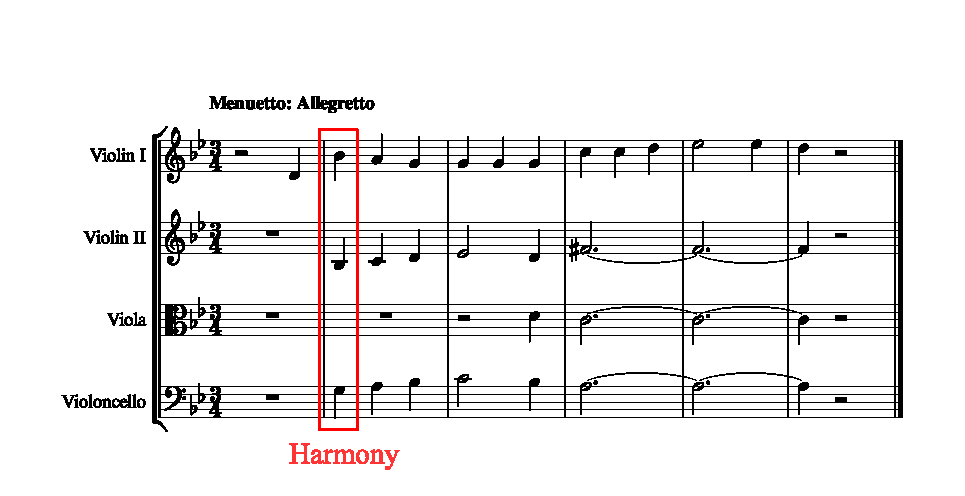
\includegraphics[width=1.0\textwidth]{01-introduction/figures/1}
\end{figure}

Combining these definitions, one possible interpretation of what is a harmonic analysis could be the following:

\begin{quote}
\centering
\emph{[...] the interpretation of \textbf{harmonic} structures in music, \linebreak
their resolution into relatively simpler elements, \textbf{i.e., harmonic labels}, \linebreak and the investigation of the relevant functions of those \textbf{labels}.}
\end{quote}

\begin{figure}[h]
  \caption{Highlighting harmonic structures in musical excerpt}
  \label{fig:harmonic-structures}
  \centering
    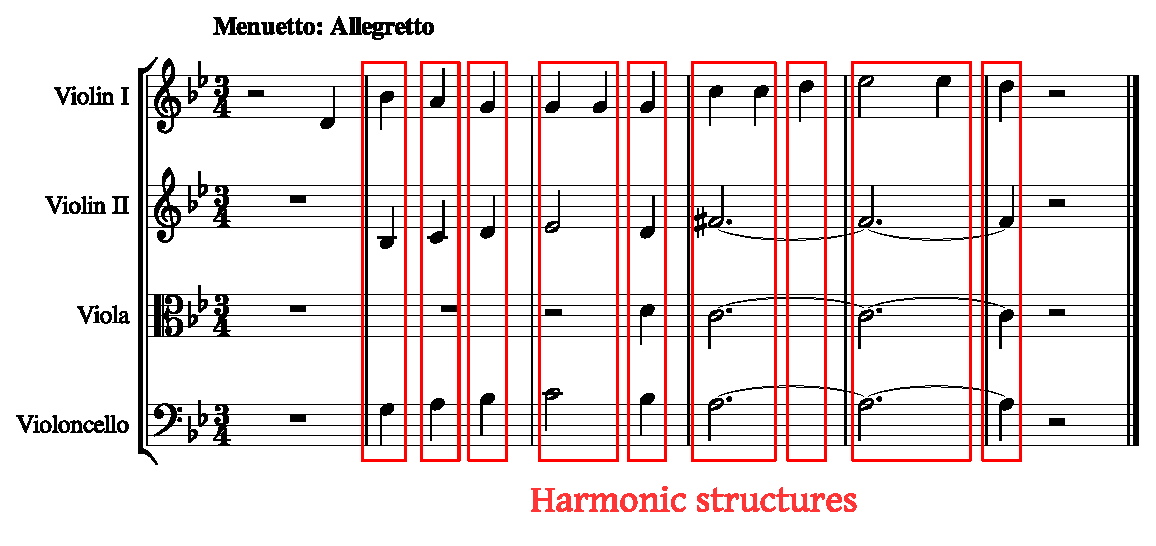
\includegraphics[width=1.0\textwidth]{01-introduction/figures/2}
\end{figure}

Therefore, as stated by this definition, the process of harmonic analysis comprises three steps:

\begin{itemize}
  \item Interpreting the harmonic structures in music
  \item Resolving these harmonic structures into harmonic labels
  \item Investigating the relevant functions among these labels
\end{itemize}

For breaking down the steps of the analysis, we could use a fragment of a musical score. Figure \ref{fig:harmony} remarks the first beat of the second measure, where three instruments play notes together. Every instance of this simultaneities represents harmony. If these harmonies are clustered and interpreted, we come up with harmonic structures, as in Figure \ref{fig:harmonic-structures}

In order to satisfy the second step of harmonic analysis, we could resolve this interpretation of harmonic structures into some sort of simpler representation. Historically, music theorists performing these sort of harmonic analysis will most likely come with a system of labels that represent the meaning of a harmonic structures. There is not a single labeling system for this purpose. Figure \ref{fig:harmonic-labels} shows three possible representations for the harmonic structures of the same music excerpt presented previously.

\begin{figure}[h]
  \caption{Three different harmonic labeling representations of a musical fragment}
  \label{fig:harmonic-labels}
  \centering
    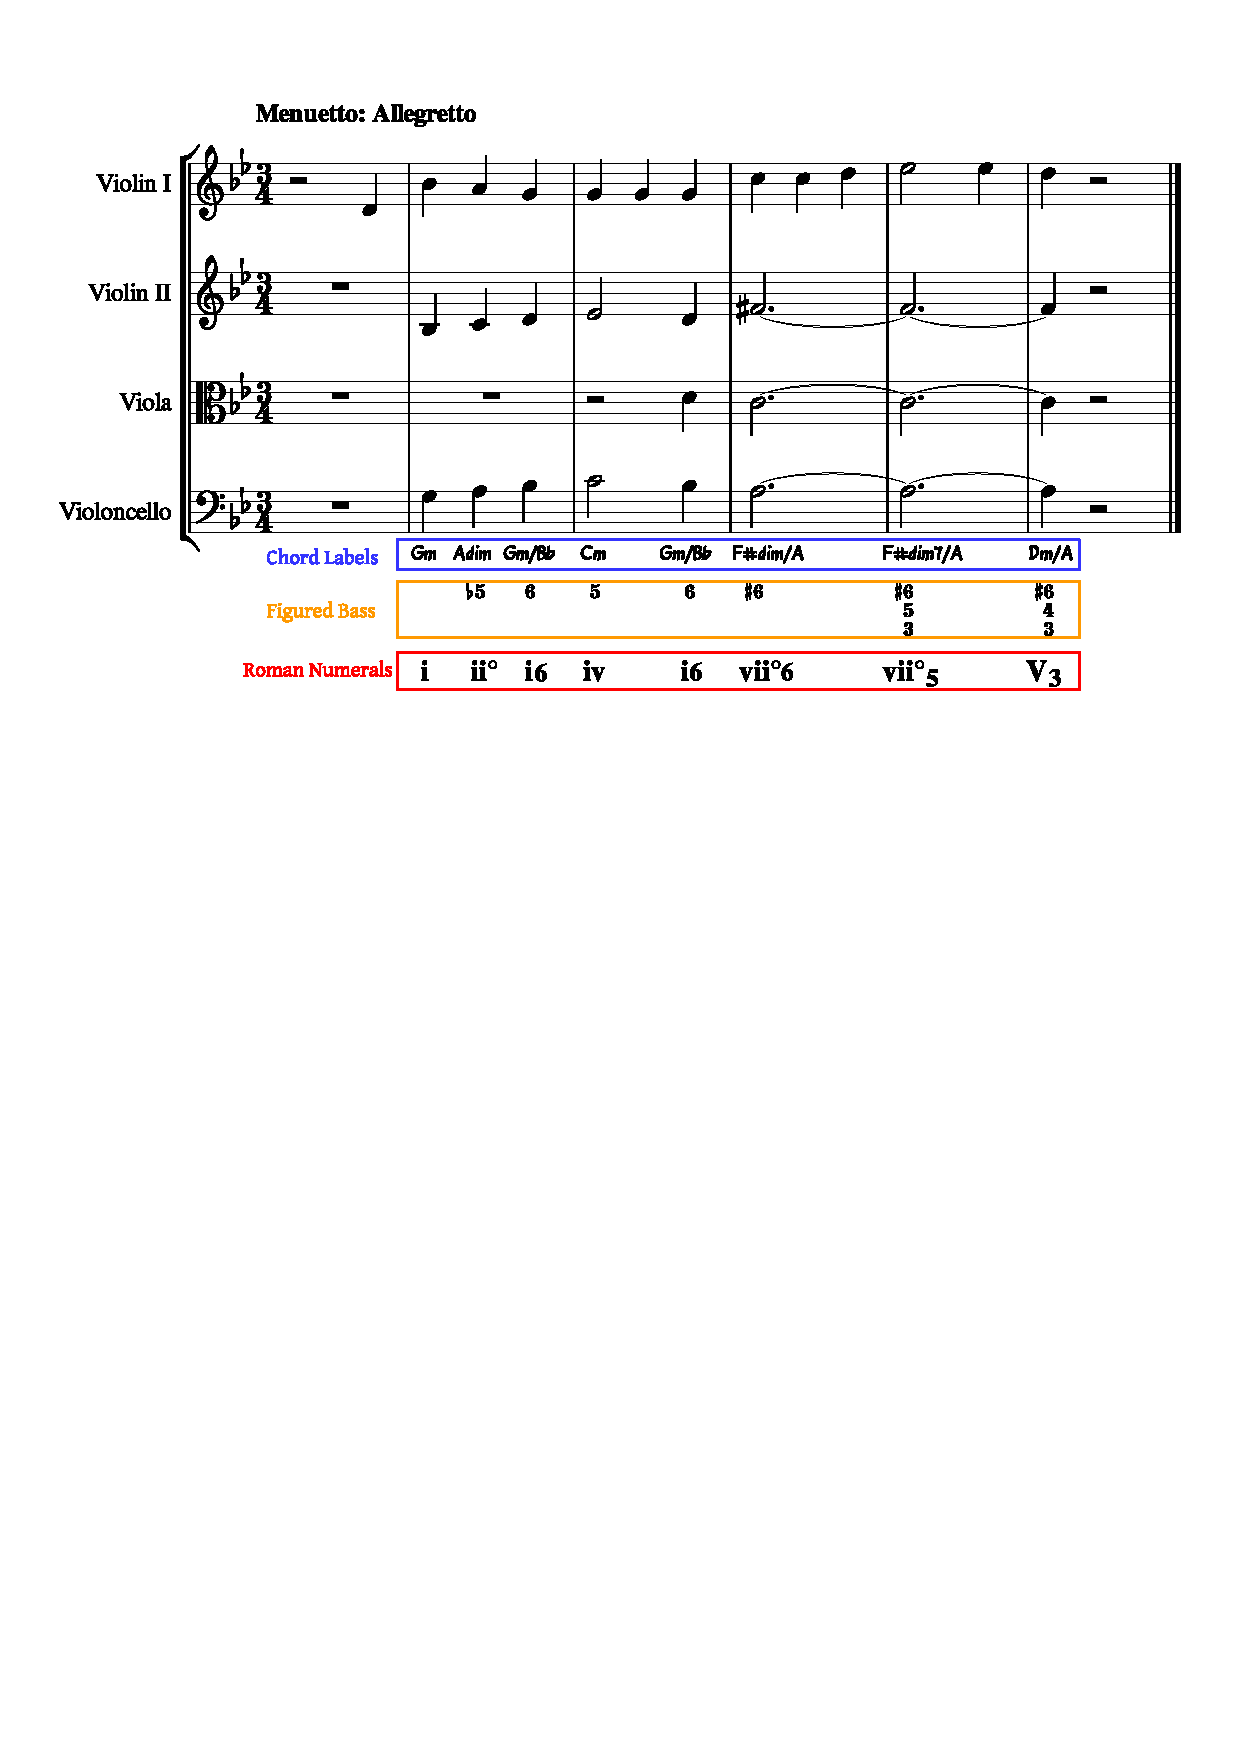
\includegraphics[width=1.0\textwidth]{01-introduction/figures/3}
\end{figure}

Any of these three representations would suffice the second step of harmonic analysis. The chord labels in the first representation are what is commonly seen to label harmonic structures in Jazz and pop music. The figured bass from the second representation was very popular previous to the classical period, and it was intended to aid accompanyists who played in chamber ensembles, e.g., it helped a harpsichordist to "fill-in" the accompaniment during the performance when only one note was given in the score. The third representation using roman numerals emerged previously but consolidated with the theoretical work of Hugo Riemann, and its purpose is mainly of analysis. For this work, I have selected to use the third kind of representation. Further discussion of this harmonic representations is given in the literature review section.

\section{Motivation}
The main reason why it would be benefical for musicians and musicologists to automate a harmonic analysis is because it takes a considerable amount of time and knowledge to perform these analyses. In practice, students at conservatoires often learn the guidelines of harmonic analysis during a specialized course of Harmony. Such a course could extend to several years, making it a difficult discipline to learn fast for a beginner. Even in the case of experts, it might take relatively long time to analyze a piece of music in terms of harmony, which makes the task of automating it valuable even for the expert theorist.

\section{Objectives}
This work pretends to reproduce and apply the current approach for automatic functional harmonic analysis used over the KernScores corpora, and apply it to a specific set of string quartets from Joseph Haydn. Once these automatic analyses are performed, they will be compared to manual annotations over the same set of string quartets.

\section{Structure of the Report}
Literature. Methods. Results. Discussion.

\newpage


% Description of the dataset
\chapter{Dataset}
\label{chap:dataset}
The dataset used for this work is a novell dataset created as part of the final output of this work. It consists of 24 musical scores corresponding to six string quartets, Op.20, written by Joseph Haydn. These quartets are commonly known as the \emph{Sun quartets}.

\begin{table}[]
\centering
\begin{tabular}{|l|c|c|c|}
\hline
Number & Movement & Tempo & Musical form \\ \hline
\multicolumn{4}{|l|}{Op.20 No.1} \\ \hline
1 & I & Allegro Moderato & Sonata \\ \hline
2 & II & Minuetto. Allegretto & Minuet \\ \hline
3 & III & Affettuoso e sostenuto & Aria \\ \hline
4 & IV & Finale. Presto & Allegro \\ \hline
\multicolumn{4}{|l|}{Op.20 No.2} \\ \hline
5 & I & Moderato & Sonata \\ \hline
6 & II & Adagio & Aria* \\ \hline
7 & III & Minuetto. Allegretto & Minuet \\ \hline
8 & IV & Fuga a 4 Soggetti & Fuga \\ \hline
\multicolumn{4}{|l|}{Op.20 No.3} \\ \hline
9 & I & Allegro con Spirito & Sonata \\ \hline
10 & II & Minuetto. Allegretto & Minuet \\ \hline
11 & III & Poco Adagio & Aria \\ \hline
12 & IV & Finale. Allegro Molto & Sonata \\ \hline
\multicolumn{4}{|l|}{Op.20 No.4} \\ \hline
13 & I & Allegro di Molto & Sonata \\ \hline
14 & II & Un poco Adagio Affettuoso & Theme and variations \\ \hline
15 & III & Allegretto alla zingarese & Minuet \\ \hline
16 & IV & Presto scherzando & Sonata \\ \hline
\multicolumn{4}{|l|}{Op.20 No.5} \\ \hline
17 & I & Allegro moderato & Sonata \\ \hline
18 & II & Minuetto & Minuet \\ \hline
19 & III & Adagio & Siciliana \\ \hline
20 & IV & Finale: Fuga a due Soggetti & Fuga \\ \hline
\multicolumn{4}{|l|}{Op.20 No.6} \\ \hline
21 & I & Allegro di Molto e Scherzando & Sonata \\ \hline
22 & II & Adagio, Cantabile & Sonata \\ \hline
23 & III & Minuetto. Allegretto & Minuet \\ \hline
24 & IV & Fuga a 3 Soggetti. Allegro & Fuga \\ \hline
\end{tabular}
\caption{The 24 music pieces within Haydn's Op.20}
\label{table:op20}
\end{table}

The comprehensive works included in Op.20 is listed in \autoref{table:op20}, as can be seen, among these 24 pieces there are several sonata, fugues, minuets, theme and variations and aria musical forms. This variety of musical forms was one important reason to create a harmonic analysis dataset out of these string quartets.

The dataset lies in the following repository \url{https://github.com/napulen/haydn_op20_harm}.

\section{String quartet}
String quartets are one of the most prominent genres developed during the Classical period. For composing in this genre, a broad knowledge of harmony is required.

In terms of harmonic analysis, string quartets are interesting as they provide four voices for most of the time, which is the number of voices in which harmony is usually taught and studied. Additionally, in the symbolic representation of the music, it is more likely that each voice will be separated in a different channel (or spine, in the case of humdrum), which is an additional aid to the harmonic analysis algorithms, as melodic seggregation is an important problem seen in these algorithms.

\section{Joseph Haydn}
Joseph Haydn is colloquially named \emph{The father of the string quartet}. He represents a major figure of the classical period of western art music,
exemplifying many of the characteristic features of the style. Also, he was a mentor for two other major figures of the classical period, Wolfgang Amadeus Mozart and Ludwig van Beethoven.

\section{Op.20 String quartets}
The \emph{sun quartets} provided to be representative works of the string quartet genre, while remaining innovative to the compositional technique of string quartets. Among the reasons to use them in this work stands the interesting distribution of musical forms in their movements. As displayed in \autoref{table:op20}, within these string quartets there are sonata form movements, fugues, theme and variations, minuets and arias.

These string quartets also remain less experimental than later works, e.g., Op.33, which makes the task of automatic harmonic analysis suitable, without adding any further complications. Finally, musical resources such as syncopation, modulation, imitation and counterpoint are handled with mastery along these 24 pieces, which introduces different scenarios and test cases for an automatic harmonic analysis algorithm.

\section{Creating the dataset}
\subsection{Extending KernScores content}
In order to create the dataset used in this work, I based in the current symbolic scores that can be found in the \href{http://kern.ccarh.org/}{KernScores} website \cite{kernscores}. This website already hosts 19 out of the 24 humdrum scores comprehending the Op.20 string quartets, so the effort left for having the entire Op.20 is to transcribe the musical pieces shown in \autoref{table:missing-op20} in a similar symbolic representation:

\begin{table}[]
\centering
\begin{tabular}{|l|}
\hline
Missing movement \\ \hline
Op.20 No.1 - III. Affettuoso e sostenuto \\ \hline
Op.20 No.2 - II. Adagio \\ \hline
Op.20 No.3 - I. Allegro con Spirito \\ \hline
Op.20 No.4 - I. Allegro di Molto \\ \hline
Op.20 No.4 - II. Un poco Adagio Affettuoso \\ \hline
\end{tabular}
\caption{Missing scores from Op.20 that are not available in the KernScores website}
\label{table:missing-op20}
\end{table}

\subsection{Manual annotations}
Once the symbolic scores are complete, the next step in the creation of the dataset involves a manual harmonic analysis of each of the pieces. As presented during \autoref{chap:introduction}, the expected output of the system is an annotated version in the form of a roman numeral analysis. Therefore, the manual analysis performed over the 24 pieces of the dataset have been done using this roman numeral analysis labeling as well.

The best way to digitally append a roman numeral analysis to these symbolic scores is using the \emph{**harm} \cite{harm} syntax, which can be included as a spine in the humdrum file. \autoref{table:manual-annotation} shows an example of appending this manual roman numeral analysis to the same excerpt of music presented since the beginning of this document, i.e., \emph{Joseph Haydn's Op.20 No.3 - II. Menuetto: Allegretto, mm.1-6}.

\begin{table}[]
\centering
\begin{tabular}{|llll|ll|}
\hline
\multicolumn{4}{|l|}{Original humdrum score} & \multicolumn{2}{l|}{Appended analysis} \\ \hline
**kern & **kern & **kern & **kern & **harm & **commentary \\
*k{[}b-e-{]} & *k{[}b-e-{]} & *k{[}b-e-{]} & *k{[}b-e-{]} & *k{[}b-e-{]} & *k{[}b-e-{]} \\
*g: & *g: & *g: & *g: & *g: & *g: \\
*clefF4 & *clefC3 & *clefG2 & *clefG2 & * & * \\
*M3/4 & *M3/4 & *M3/4 & *M3/4 & *M3/4 & *M3/4 \\
2r & 2r & 2r & 2r & . & . \\
4r & 4r & 4r & 4d & . & . \\
1 & 1 & 1 & 1 & 1 & 1 \\
4G & 2.r & 4B- & 4b- & i & . \\
4A & . & 4c & 4a & iio & \begin{tabular}[c]{@{}l@{}}Not really diminished, \\ missing the fifth\end{tabular} \\
4B- & . & 4d & 4g & ib & . \\
2 & 2 & 2 & 2 & 2 & 2 \\
2c & 2r & 2e- & 4g & iv & . \\
. & . & . & 4g & . & . \\
4B- & 4d & 4d & 4g & ib & . \\
3 & 3 & 3 & 3 & 3 & 3 \\
{[}2.A & {[}2.c & {[}2.f\# & 4cc & viiob & . \\
. & . & . & 4cc & . & . \\
. & . & . & 4dd & V7c & . \\
4 & 4 & 4 & 4 & 4 & 4 \\
2.A\_ & 2.c\_ & 2.f\#\_ & 2ee- & viioD7b & . \\
. & . & . & 4ee- & . & . \\
5 & 5 & 5 & 5 & 5 & 5 \\
4A{]} & 4c{]} & 4f\#{]} & 4dd & V7c & . \\
2r & 2r & 2r & 4r & . & . \\
. & . & . & 4d & . & . \\ \hline
\end{tabular}
\caption{Example of appending a manual annotation of roman numerals to a humdrum score}
\label{table:manual-annotation}
\end{table}





\newpage


% Literature review
\chapter{Literature review}
\label{chap:literature-review}
Most researchers agree that the pioneer work addressing the problem of harmonic analysis is the approach made by Terry Winograd in 1968 \cite{winograd1968linguistics}. Since then, researchers have developed over the idea of harmonic analysis in very different ways.

One possible reason for this is how much the harmony of different kinds of music diverges. Even restricting ourselves to tonal music, we would still comprehend a range of music as wide as late 16th century's Claudio Monteverdi to 20th century fusion jazz' Allan Holdwsworth. It is very difficult to imagine an automatic harmonic analysis approach that could serve all sorts of music and at the same time deal with the details, common practices and corner cases from these different music styles and periods.

Therefore, in practice, researchers have systematically split their efforts to target specific kinds of music, and even sometimes, specific composers. One example of that is this work itself, which runs automatic harmonic analyses over music from the classical period of Western art music, composed by Joseph Haydn and no other composer.

 However, I believe that interesting insight to the task of automatic harmonic analysis can be derived from the methods used in different kinds of music, particularly jazz. These observations are useful for the better understanding of key aspects of the problem of harmonic analysis, related even to the music of Joseph Haydn and composers alike.

 \section{Jazz harmonic analysis}
 After Winograd, probably one of the pillar works in harmonic analysis for jazz is that of John Wade Ulrich \cite{ulrich1977analysis}. This work developed a functional analysis, identifying the function of each chord in a musical piece. The input for this model was a sequence of chords and it incorporated the detection of keys. Among some of the restrictions it has is that it does not work for music in a minor tonality, and constraints chord changes to occur once every beat.
 Following to the model from Ulrich, probably one of the next pillars in harmonic analysis oriented to jazz music and a direct successor to the baseline of Ulrich is the model from Francois Pachet \cite{pachet2000computer} who presents a hierarchical model to analyze jazz harmonic progressions, similarly taking as input a sequence of chords and deriving a hierarchical description of modulations. This model does not consider voice-leading and lands in the more "hierarchical" type of analysis, which give structure to a set of chord labels. It was later extended by Ricardo Scholz \cite{scholz2005automating} who attempted to incorporate modal borrowings and secondary dominants.

 From these research, we can infer an important fact, most of the jazz oriented approaches lie within the context of \emph{hierarchical} approaches to functional harmony, and oftenly trivialize the input to chord labels to focus on the functional hierarchies themselves. One of the most important problems in classical music, for example, is precisely in how to deal with all these melodic streams before they can be considered chord labels. This happens maybe because the harmonic movement in Jazz is much more aggressive and departs from a tonal center with ease, making the effort of tracking fast-moving tonal centers an attractive problem, and melodic, polyphonical implications of the music less useful, whereas in classical music it is usual to well-establish one tonal center before moving to the next, at least for the classical period, but extracting the implied tonal function within the different melodic streams is not a trivial task to solve. These characteristics of the music styles probably point out and justify the motivations for separating the models according to the music that is being analyzed.

 As the target music of this work belongs to the early Classical period in western art music, I will be dealing with the approaches concerning this kind of music, with special attention to those approaches that attempt to solve the problem entirely, without assuming an input of chord labels, but a full musical score.

 Once established that this work is dealing with music from the Classical period and therefore its interest is in the approaches that attempt to provide an automatic harmonic analysis of such subset of tonal music, I will start to describe some of the remarkable efforts done, putting special emphasis to their contributions, inputs, outputs and flaws.

\section{Automatic harmonic analysis}

    \subsection{The pioneer work by Terry Winograd}
    As it was stated before, researchers in the field mostly mention the approach from Terry Winograd, in 1968, as the pioneer work in the field. This work is not only important because it is the first and pioneering work in computing a functional harmonic analysis, but also because it linked the computational techniques used in natural language processing to music. The model from Winograd was evaluated over music from Johann Sebastian Bach, and pretends to output a functional harmonic analysis of such pieces of music. To provide an output, it requires a preliminary hand-made conversion of the original score and turn it into a sequence of four-part perfect chords. This allowed him to process a score using his implementation in the LISP programming language, but it also means that during this pre-processing stage the non-harmonic tones are eliminated before solving the problem. In his 1997 harmonic analysis algorithm \cite{temperley1997algorithm}, David Temperley provided insight about the flaws of Winograd's model, among them he mentions the issues concercing melodic seggregation and arpeggiations.
    \subsection{Expert system from Maxwell}
    A direct successor of Winograd's approach, the model from John Maxwell, which was part of his PhD dissertation in 1984, and successively published in 1992 \cite{maxwell1992expert}, is probably the best example of the rule-based approaches towards harmonic analysis. Same as Winograd, Maxwell's target was to output a functional harmonic analysis from a music score. The model from Maxwell has fifty five rules that pretend to reduce the vertical sonorities into a chord sequence, and then deciding for key changes. Some of the rules are intuitive and basic, e.g., \emph{"Perfect and imperfect consonant intervals constitute a consonant interval. Every other is a dissonant interval."}, while others appear cryptic and difficult to understand, e.g., \emph{"If the goal chord falls on a strong beat and it is a major triad or major-minor seventh, and the root movement from the pre-cadence is an ascending or descending perfect fifth or major second or a descending minor second, and when the root motion is a descending fifth, the pre-cadence is not a potential dominant, and when the root motion is an ascending fifth the pre-cadence is triadic, then the pseudo-cadence is a half cadence, and its strength increases by 10."}.
    The later rule also reveals a problem that was pointed out by future researchers, the use of arbitrary, fixed values while determining the strength of a cadence. Even so, the results of Maxwell's approach get really close to the outcome expected by a music theorist analyzing a music score and determining its functional harmony. This work was tested over three different movements of Johann Sebastian Bach's Six French Suites: The sarabande from Suite No.1, the menuet from Suite No.2 and the gavotte from Suite No.5. The pieces selected comprehend different problems and levels of complexity to be addressed: Four-part harmony with several non-harmonic tones, 2-voice continuous contrapuntual movement, and a varying contrapuntual texture, respectively. David Temperley put the limitations of Winograd and Maxwell's approaches pretty close together, summarizing them in the following:
		\begin{itemize}
			\item Sequences of notes that are not displayed simultaneously (vertically), as arpeggiations of chords.
			\item Missing pitches in the spelling of a full chord, which can be deduced from the context.
			\item Ornamental notes. Maxwell proposes specific rules to deal with these notes, but according to Temperley, neither Maxwell's or Winograd's are good enough to correctly detect ornamental notes.
    \end{itemize}
    Maxwell's approach, in general, represents the powerful and sophisticated machinery of rule-based approaches, as well as their complexity.
    \subsection{Temperley and the Melisma Music Analyzer}
    Probably the most relevant approach in automatic harmonic analysis for this work, is the approach from David Temperley described in 1997 \cite{temperley1997algorithm}, as it was extended afterwards by his work in key estimation algorithms and which culminated in the implementation of the Melisma Music Analyzer, in conjunction with Daniel Sleator.
    Inspired by the cognitive experiments by Carol Krumhansl \cite{krumhansl2001cognitive}, the aim of Temperley is to produce an algorithm that models the human process of harmonic analysis done by a trained expert, and to take it as indicative of the analysis produced subconsciously by listeners in general.

		The traiditional functional harmonic analysis done in music theory courses uses the \emph{roman numerals} notation to segment a piece of music, labeling it with symbols indicating the relationship between each root to the current key. Temperley steps forward in the definition of the problem of harmonic analysis, decomposing the task into two subtasks: \emph{root finding} and \emph{key finding}. Temperley claims then that functional harmonic analysis could be broken down into these subtasks, focusing at first in root finding, assuming that this task can be done independently to key finding. Root finding basically consists of dividing a piece into segments and label each of them with a root.

    Once in the task of root-finding, Temperley approaches the task defining certain rules: \emph{Pitch variance rule, compatibility rule, strong-beat rule, harmonic variance rule and ornamental dissonance rule}. Together with these rules, he introduces important definitions that aid in the process of root analysis: The concepts of \emph{Tonal Pitch Class} (TPC), \emph{Center of Gravity} (COG) and the \emph{line of fifths}.

    It is difficult to follow the chronology of this approach, as the implementation of this model comes mainly in the form of the Melisma Music Analyzer, which was released in 2001, and included the key estimation algorithm and a combined mode that eventually performed the complete functional harmonic analysis. The latest mode being the core implementation of what will be used to compute automatic harmonic analysis during this work.

    \subsection{Probabilistic and statistical approaches}
    Temperley himself, after the release of the Melisma Music Analyzer, moved into the direction of probabilistic models. In his case, using a Bayesian approach that aims to provide a unified modeling of harmonic analysis, meter induction and melodic seggregation, challenging the individualization of these problems without considering the connections among them \cite{temperley2009unified}.

    However, previous to this work, an important probabilistic approach that emerged to solve the problem of functional harmonic analysis was that of Christopher Raphael \cite{raphael2003harmonic}.
    This model from Raphael is one of the few pure-functional harmonic analysis approaches, oriented towards the analysis of common-practice music. The idea is simple and some of his assumptions simplify the parameters of the model. Some constant that remains as in previous models is the fact that it gets rid of all the pitch-spelling information and replaced for solely pitch information. This model, unlike Temperley, does not try to reconstruct the pitch spelling information back by any algorithmic means, and in the words of Raphael, it is an obvious extension to the model.

    Another quite important effort in the statistical domain includes the work from Martin Rohrmeier \cite{rohrmeier2008statistical}, who uses a heuristic method of segmentation. Analyzes distributions of single pitch-class-sets, chord classes and pitch-class-sets transitions. One of the goals of Rohrmeier was the research of \emph{syntacticality} in harmony. The final goal is to produce descriptive analyses of harmonic structure based on an empirical approach. The choice of the corpus is, similarly to others, music from Joahann Sebastian Bach. In his case, chorales, because they constitute a large and coherent set of pieces regarding style and composition technique. Rohrmeier claims that this work is pioneer in the statistical analysis of a corpus for the purpose of finding features of tonal harmony. According to the results of Rohrmeier, the most frequent occurrences of pitch-class-sets in this music are those of tonic, dominant and subdominant chords. This would be expected and helps to reinforce those scale-degree theories that describe harmonic movement with transition tables of scale degrees. The results from this research, apart from being interesting in confirming music-theory beliefs regarding common chords and transitions in tonal music, could also be replicated in a different corpus to target its particular common chords and transitions.

    \subsection{Grammar-based}
    Three years after his statistical work in Bach Chorales, Martin Rohrmeier brought back the use of grammars to study the underlying structure of musical harmony \cite{rohrmeier2011towards}, which inspired future works by other researchers in the field, specially towards analyzing jazz music. In this work, Rohrmeier claims that the structure of harmonic progressions exceeds the simplicity of a markovian transition table, and he proposes a set of phrase-structure grammar rules. For this purpose, the hierarchical analysis from the music-theory approach done by \cite{kostka1995tonal} is presented, with the belief that it can be brought to a closer formalization. Rohrmeier presents a tree representation of a chord sequence, using two principles:
    \begin{itemize}
			\item Chords have dependencies and the existence of one sometimes requires the existence of another
			\item Chords have functions, these functions can be realized by a set of chords.
		\end{itemize}
    The system comprises 27 rules for the generation of a grammar, this helps to model common-practice music as well as jazz music. The output of this algorithm is a hierarchical tree of the functions and dependencies of the chords. The level of detail from this work to model every special case of the harmonic language is remarkable, as careful attention has been put trying to comprehend distinct kinds of cadences, chords and modulations in the model.

    This work was eventually retaken and implemented by Bas de Haas \cite{de2013automatic} using chord labels as input for the system.

    As discussed previously, different methods of performing harmonic analysis oftenly have different outputs in mind, considering this, I will mention that even if the hierarchical representations of harmony appear interesting and promising, the aim for this work is to provide music scores as input and produce an automatic harmonic analysis as output. In this sense, the most relevant approaches can be reduced simply to those approaches who pretend to output exactly that.

  During \autoref{chap:introduction}, I presented three different label sets as the harmonic analysis of a fragment of music, this appears in \autoref{fig:chord-labels}. It is important now to mention the selected labeling system, as this influences the approach to be chosen for this work.

  \section{Labeling harmonic structures}
  Harmonic analysis could be seen from different perspectives, the first one I would like to address is how it was conceived and modeled by music theorists. Starting with the french composer Jean-Philippe Rameau (1683-1764), until the theory from the german theorist Hugo Riemann (1849-1919) in the late nineteenth century.
    \subsection{Fundamental bass}
    The original idea by Rameau was based on the movement of the bass note, the so called \emph{Fundamental Bass}, which constructed rules and principles of how the movement of a bass note determined also the movement of the harmony. Rameau's theory limited the dictionary of chords to triads and some special cases of seventh chords, and considered chord inversions for the first time, from which the core concept of harmonic root arises and suggests that the bass note could be serving a harmonic root located in the superior voices. This theory is pioneer in separating the melodic movement and coincidence in time from counterpoint \cite{beach1974origins}, and looking at the music from a vertical perspective, a vision that spread in the following periods of western art music.
    \subsection{Root succession tables}
    These set of theories, denomined by Tymoczko as \emph{scale-degree} theories \cite{tymoczko2001root}, assign a number to each of the degrees in a scale, which represents its triad, and then trying to infer the most common succession of that particular scale degree to another. This theories have been used commonly in Harmony text books, and in principle, the scale-degree transitions have not been obtained scientifically. However, due to the probabilistic nature of these theories, there have been recent efforts in validating their statements and accuracy using computational resources, such as first-order Markov models.
    \subsection{Functional harmony}
    In 1893, Hugo Riemann presented his \emph{Vereinfachte Harmonielehre}, which placed together ideas and theories from himself and earlier theorists, and gave birth to what is called \emph{Functional Harmony}. The most notable, and allegedly controversial, characterization that comes from the functions theory, is the idea of categorization of chords. Functional harmony considers that chords belong to one of three tonal functions:
    \begin{itemize}
      \item Tonic
      \item Subdominant
      \item Dominant
    \end{itemize}
    These functions contain all individual chords, but are essentially represented by the primary triads: I, IV and V.
    Due to this categorization of chords, functional harmony contains more information about tonal contexts and semantics, and therefore, as an analysis output becomes more interesting than fundamental bass or root succession theories.

  \subsection{Functional harmonic analysis}
  From the previously mentioned efforts of harmonic analysis, those that explicitly pretend to output a functional harmonic analysis from a music score, are the following:
  \begin{table}[tbp]
    \centering
    \caption{Automatic functional harmonic analysis approaches}
    \label{my-label}
    \begin{tabular}{llll}
      Approach & Year & Implementation & Availability \\
      Winograd & 1968 & LISP & No \\
      Maxwell & 1992 & LISP & No \\
      Temperley & 1997\footnote{The span of time between this approach was presented as a paper and the current implentation used for this work, is much wider, reaching changes in code done during 2017} & C & Yes \\
      Raphael & 2003 & C & Partial \\
      Illescas & 2008 & Java & Partial
    \end{tabular}
  \end{table}
  From the approaches shown in Table 1, results evident that the decision over the approach used as the baseline for this work performing an automatic harmonic analysis is that of David Temperley, which is related to the Melisma Music Analyzer. Simply put, because it is the most mature approach in terms of reproducibility and applicability to large volumes of music, like the string quartet dataset used in this work.

\newpage


% Methodology
\normallinespacing

\chapter{Methodology}
\label{chap:methodology}

As I described during \autoref{chap:literature-review}, the original model from David Temperley divided a system of automatic harmonic analysis in two subsystems: One that performs root detection and another one that performs key detection. \autoref{fig:software_stack1} shows how the core harmonic analysis of David Temperley comprises these two tasks.

\begin{figure}[ht]
  \centering
    
\includegraphics[width=0.5\textwidth]{04-methodology/figures/1}
  \caption{Harmonic analysis as divided by David Temperley}
  \label{fig:software_stack1}
\end{figure}

However, thanks to the implementation work that has been already done by David Temperley, Daniel Sleator and Craig Sapp, the idea of using an implementation of this automatic harmonic analysis system over the dataset described in this work, which consists of musical scores encoded in humdrum files, is already feasible. During this chapter I will introduce the software stack, programs and scripts that allow for running an automatic harmonic analysis of a humdrum music score.

I will start from the analysis programs of the Melisma Music Analyzer, which are the core of the analysis, to the scripts and programs of the Humdrum Extras software tools that allow for the use of real humdrum music scores.

\section{The Melisma Music Analyzer}
  The Melisma Music Analyzer was implemented by Daniel Sleator over the work of David Temperley. It takes as input a \emph{Notefile}, which could be said to be a plain-text representation of midi files. The Melisma Music Analyzer consists of several standalone programs, therefore, the output depends on the program that is being run over the \emph{Notefile} input file. However, generally speaking, they all output a plain-text analysis of some sort.

  In order to obtain a harmonic analysis, a Notefile needs to go through 3 stand-alone programs, one after another: Meter, Harmony and Key.

  \begin{figure}[ht]
    \centering
      
\includegraphics[width=1.0\textwidth]{04-methodology/figures/2}
    \caption{Melisma Music Analyzer, from a Notefile to a plain-text analysis}
    \label{fig:software_stack2}
  \end{figure}

  \subsection{Meter}
    This program extracts metrical information about the musical piece, using the theories of the Generative Theory of Tonal Music as a basis.
    The output of this program is the same notefile with beat information appended at the end.
  \subsection{Harmony}
    This program takes as input the notefile with beat information (the output from the meter program), and outputs information about harmonic roots for each beat. The name is somehow misleading, as this program's output is not harmony, but a harmonic root. Temperley divided the task of harmonic analysis in root estimation and key estimation, this program computing the first of these subtasks.
  \subsection{Key}
    This program takes as input the notefile with beat and harmonic-root information (the ouput from the harmony program). Something to remark about this program is that it might work with or without the information of the harmony program. In the first case, it performs a complete harmonic analysis. In the second case, it will only perform a key estimation.

    \autoref{fig:software_stack2} shows the flow from an input Notefile to the plain-text analysis that is being output by the key estimation program of the Melisma Music Analyzer.

  \subsection{Problems with processing Notefile files}
    The input format from the Melisma Music Analyzer, yet it resembles a midi file, it is not a midi file. It is also not a standard type of file that could be encountered typically in other software. More important, it is incompatible with the humdrum encoding of the dataset used for this work, so at this point, we are unable to run an analysis over these musical scores.

    However, there is one way around this problem. Using one of the programs found in the \emph{Humdrum extras} collection.

\section{Humdrum extras}
  The humdrum extras are a set of tools developed by Craig Sapp, mainly in the C++ programming language \cite{humextra}. These tools are useful for additional processing of musical scores encoded in humdrum. For this work, I am particularly interested in a few of these utilities that help to pass a humdrum file to the melisma music analyzer, and then bring the output from melisma back to a humdrum representation.

  \begin{figure}[ht]
    \centering
      
\includegraphics[width=1.0\textwidth]{04-methodology/figures/3}
    \caption{Automatic harmonic analysis of a humdrum musical score}
    \label{fig:software_stack3}
  \end{figure}

  The first step is mitigating the problem around the Notefile format, for this, the \emph{kern2melisma} program from the Humdrum Extras collection results quite useful.

  \subsection{kern2melisma}
    This program provides a parser to convert a humdrum file into the \emph{Notefile} format used by Melisma. It is the first step in the workflow of a functional harmonic analysis from a humdrum score.

  Once the input file is able to be processed over the programs of the Melisma Music Analyzer, it will be possible to obtain the plain-text analysis of the \emph{Key} program. However, this analysis is difficult to parse as it is. Luckily, there is already a tool from the Humdrum Extras that provides help parsing this analysis, this tool is the \emph{key2humdrum} script, written in PERL.

  \subsubsection{key2humdrum}
    This program takes the output from the \emph{Key} program and outputs a pseudo-humdrum representation.

  \subsubsection{Appending to a humdrum file}
    The last step in getting the information back into a humdrum file is parsing the output of the key2humdrum program and appending this information to a humdrum spine. This process is not done by a standalone program, but rather a program that comprehends all the process described during this chapter. This program is called \emph{tsroot}.

  \subsubsection{tsroot}
    The tsroot programs performs all the steps described before, starting from calling the \emph{kern2melisma} to calling the Melisma programs and \emph{key2humdrum}. Additionally, this program also interprets the output of key2humdrum and produces a final humdrum score with the analysis information appended to it.

    \autoref{fig:software_stack3} could be seen as the process that happens each time the \emph{tsroot} program is run over a humdrum score. This is a truthful realization of the target system for automatic harmonic analysis explained in the first chapters of this document.

\newpage


% Results
\chapter{Results}
\label{chap:results}

\section{Best performance}
\begin{itemize}
  \item Op.20 No.5 - III: 85.49\%
\end{itemize}
\section{Worst performance}
\begin{itemize}
  \item Op.20 No.5 - III: 15.89\%
\end{itemize}
\section{Helen Budge chord frequencies}
\section{Comparison against it}
\section{Performance tables per score}
\newpage


% Conclusion and Discussion
\chapter{Discussion}
\label{chap:discussion}

\section{Conclusions}

\section{Future work}
  \subsection{Musical domain}
    \subsubsection{Beethoven Op.18}
    \subsubsection{Mozart Op.10}
  \subsection{Technological domain}
    \subsubsection{Focusing in scores}
    Leaving cognition behind
    \subsubsection{Pitch-spelling}
    Illescas has done it, but none else

\newpage


\listoffigures
\newpage
\listoftables

% appendices come here
\bibliographystyle{naturemag}
\bibliography{bibliography}

\appendix
\chapter{Issues} %Appendix A
This section describes different issues presented and addressed during this work
	\section{Transcription issues}
		\subsection{Transcription of the missing files from Op.20}
    \begin{itemize}
    \item Op.20 No.4 - I: mm.127
		Replacing E in the first beat of the second violin, for E\#
    \end{itemize}
    \subsection{Corrections over the Altmann Edition}
    \begin{itemize}
    \item Op.20 No.2 - I: mm.29
    In the Altmann edition, the bass goes to E flat after a Dominant Seventh chord, however, in other editions it moves to the tonic, it makes more sense to the harmonic context to move towards the tonic, therefore, ignoring the spelling of the Altmann Edition for this measure and considering the bass as heading to the tonic in the third beat of the measure.
    \end{itemize}
		\subsection{Corrections over previous KernScores corpus}
    \begin{itemize}
    \item Op.20 No.4 - I: mm.124
    Changing the spelling of the viola from F natural to E sharp as it explains better a dominant seventh chord, and also, it appears like that in the Altmann Edition.

    \item Op.20 No.4 - IV: mm.24
    Adding an e natural to the first violin. It matches what is written in the Altmann Edition, and it makes the harmony clearer, from a g-diminished triad to a fully diminished e natural seventh chord, which explains better the f chord in the next measure

    \item Op.20 No.4 - IV: mm.92 \& mm.94
    Correcting wrong spelling of a note in the viola

    \item Op.20 No.6 - II: mm.5
    Changing the D in the fourth beat of the measure for a B natural, which matches the Altmann Edition
    \end{itemize}
	\section{Annotation issues}
    \subsection{Corner cases}
      \begin{itemize}
        \item Op.20 No.4 - IV: mm.6 "The augmented triad on the fifth scale degree may be used as a substitute dominant, and may also be considered as bIII+, for example in C: V+ = G-B-D\#, bIII+ = Eb-G-B, and since in every key D\# = Eb, they are the same three pitches.", Theories and Practice of Harmonic Analysis. p. 35. ISBN 0-7734-9917-2.
      \end{itemize}
		\subsection{Non-expert analysis}
    Most of the analyses were done by me, I am not an expert.
		\subsection{Fugues are too contrapunctual}
    The fourth movements of Op.20 No.2, No.5 and No.6 are fugues, these were some of the most difficult scores to analyze manually, mainly because they are very contrapunctual.
		\subsection{Flat -VII annotated as VII}
    While annotating the scores, I marked the lowered seventh degree of the minor mode simply as VII, while it should be a lowered seventh -VII. It could affect the results.
	\section{Workflow issues}    
		\subsection{Source code coming from different sources}
    The main problem is that the source code comes from different repositories, and it is difficult in terms of reproducibility to put everything together in one place and guarantee it will work.
		\subsection{Melisma array sizes}
    There was an "error" in the melisma music analyzer. The size of static structures like arrays, have been hardcoded, in long scores like Op.20 No.3 - I, the program reached buffer overflow and crashed without completing the analysis, I fixed my version of the Melisma Music Analyzer programs to correct this, but this code is not public, as I am not aware of the license of the Melisma source code. If attempting to run the analysis in these files, the programs will crash unless this is fixed.
    \begin{itemize}
    \item Op.20 No.4 - IV
    \item Op.20 No.3 - I
    \item Op.20 No.5- I
    \end{itemize}
		\subsection{tsroot harmony2humdrum and key2humdrum}
    tsroot had a different default tempo than kern2melisma, therefore, when running the analysis over files with no explicit tempo information, the result is incorrect. I fixed this in my version of the humdrum extra tools, you can download it from my fork repository. At the moment of this publication, the fix for this has not been merged in the main project repository.
	\section{Evaluation issues}
		\subsection{Chr chords are ignored}
    I am ignoring the annotations denoted as \emph{Chr} by the automatic analysis, instead of denoting a change of harmony after encountering this tag, I am preserving the previous harmonic root. This is probably wrong and should be addressed in a future evaluation.
		\subsection{Resolution of degree in secondary functions}
    Though I described the process to resolve a subfunction, I did not write this code with my harmparser. In practice, I delegated this process to the harm2kern program that is already available in the humdrum extra tools. I did not check if the parser from harm2kern is doing this process as I described it. It might be somewhat different.
	\section{Bugfixes}
  As the result of this work, a few problems were addressed
		\subsection{tsroot --meldir and --midir args}
    The implementation of tsroot has a hardcoded default value of the meldir and midir directories, when trying to change it with console arguments, the program crashed as there was some issue in the translation of the C string. This problem was detected and now it is corrected in the latest version of humdrum extras. Special thanks to Craig Sapp who double-checked this after I posted in the humdrum forum
		\subsection{tsroot tempo correction}
    As stated previously, there is a different default tempo in the tsroot program than the kern2melisma program, this means if a file has not an explicit tempo indication, the output analysis is incorrect. This was the case for the entire dataset of Op.20, so detecting and correcting this issue was crucial for this work. This fix has not been until this point merged into the official humdrum extra repository.
\newpage


\end{document}
